\documentclass[12pt]{article}

\usepackage[utf8x]{inputenc} % Включаем поддержку UTF8  
\usepackage[russian]{babel}  % Включаем пакет для поддержки русского языка  
\usepackage{hyperref}        % Для гиперссылок

% Математика
\usepackage{amsmath,amsfonts,amssymb,amsthm,mathtools} % AMS
\usepackage{icomma}
\usepackage{mathrsfs}

\usepackage{xcolor}

% Прога
\usepackage{etoolbox}
\usepackage{listings}

\definecolor{codegreen}{rgb}{0,0.6,0}
\definecolor{codegray}{rgb}{0.5,0.5,0.5}
\definecolor{codepurple}{rgb}{0.58,0,0.82}
\definecolor{backcolour}{rgb}{0.95,0.95,0.92}

\lstdefinestyle{mystyle}{
	backgroundcolor=\color{backcolour},   
	commentstyle=\color{codegreen},
	keywordstyle=\color{magenta},
	numberstyle=\tiny\color{codegray},
	stringstyle=\color{codepurple},
	basicstyle=\ttfamily\footnotesize,
	breakatwhitespace=false,         
	breaklines=true,                 
	captionpos=b,                    
	keepspaces=true,                 
	numbers=left,                    
	numbersep=5pt,                  
	showspaces=false,                
	showstringspaces=false,
	showtabs=false,                  
	tabsize=2
}

\lstset{style=mystyle}

% Цвета
\usepackage{xcolor}

% Картинки
\usepackage{graphicx}
\graphicspath{ {./images/} }

\usepackage{tikzsymbols}

% Работа с таблицами
\usepackage{array,tabularx,tabulary,booktabs} % Дополнительная работа с таблицами
\usepackage{longtable}  % Длинные таблицы
\usepackage{multirow} % Слияние строк в таблице

% Нумерованные списки
\usepackage[shortlabels]{enumitem} % Разные лейблы

% Текст
\usepackage[normalem]{ulem}  % для зачеркивания текста

\newtheorem{property}{Свойство}
\newtheorem{consequence}{Следствие}[property]

\DeclarePairedDelimiter\abs{\lvert}{\rvert}%
\DeclarePairedDelimiter\norm{\lVert}{\rVert}%

% Swap the definition of \abs* and \norm*, so that \abs
% and \norm resizes the size of the brackets, and the 
% starred version does not.
\makeatletter
\let\oldabs\abs
\def\abs{\@ifstar{\oldabs}{\oldabs*}}
%
\let\oldnorm\norm
\def\norm{\@ifstar{\oldnorm}{\oldnorm*}}
\makeatother

\begin{document}
	
	\thispagestyle{empty}
	\begin{center}
		\textbf{ПРАВИТЕЛЬСТВО РОССИЙСКОЙ ФЕДЕРАЦИИ}
		
		\vspace{5ex}
		
		\textbf{Федеральное государственное автономное образовательное учреждение \\ высшего образования \\ <<Национальный исследовательский университет \\ <<Высшая школа экономики>>}
	\end{center}
	\vspace{5ex}
	
	\begin{center}
		Московский институт электроники и математики им. А.Н. Тихонова  
		
		\vspace{5ex}
		
		Департамент прикладной математики
		
		\vspace{10ex}
		\textbf{Отчёт \\ по лабораторной работе №8 \\ по курсу <<Алгоритмизация и программирование>> \\ Задание № 13}
		\vspace{7ex}
		
	\end{center}
	
	\begin{center} 
		\begin{tabular}{| p{0.3\linewidth}| p{0.3\linewidth}| p{0.3\linewidth}|}
			\hline	
			ФИО студента & Номер группы & Дата \\  \hline
			& & \\  
			Кейер Александр \newline Петрович & БПМ-231 & \today\\  
			& & \\  \hline		
		\end{tabular}
	\end{center}
	
	\begin{center}
		\vspace{3ex}
		
		\vfill
		
		\normalsize
		
		\textbf{Москва, 2023}
	\end{center}
	
	\newpage
	
	%---------------------------------------------------------------------------------
	
	\section*{Задание (вариант № 13)}
	
	\begin{enumerate}
		\item Данные должны храниться в бинарном файле.
		\item Каждая операция с данными базы должна быть реализована как функция или набор функций.
		\item Выбор и запуск требуемого режима (действия) осуществляется через меню.
		\item Реализовать следующие функции обработки данных:
		\begin{itemize}
			\item добавление записи в файл;
			\item удаление заданной записи из файла по порядковому номеру записи;
			\item поиск записей по заданному пользователем (любому) полю структуры;
			\item редактирование (изменение) заданной записи;
			\item вывод на экран содержимого файла в табличном виде.
		\end{itemize}
		\item Структуру (в соответствии с вариантом) определять в отдельном заголовочном файле. С
		помощью директив условной компиляции определить два способа ввода исходных данных в
		файл: пользователем с потока ввода и из заранее заполненного массива.
	\end{enumerate}
	
	\newpage
	
	\section*{Структура заголовочного файла}
	
	\begin{lstlisting}[language=C]
		#define fieldLength 64
		#define fieldSize fieldLength * sizeof(char)
		#define entryLength 6
		
		struct footballerType {
			char fullName[fieldLength];
			char clubName[fieldLength];
			char role[fieldLength];
			int age;
			int numberOfGames;
			int numberOfGoals;
		};
	\end{lstlisting}
	
	\section*{Решение}
	
	\begin{lstlisting}[language=C]
		#pragma once
		
		#include "football.h" // Headers file.
		
		#include <stdio.h> // Input/output library.
		#include <string.h> // String library.
		#include <stdlib.h> // Mmory allocation library.
		#include <io.h> // File managing library.
		
		#define FILE_NAME "footballer.bin" 
		#define INPUT_TYPE 'a'
		
		// Function printing horizontal line.
		void printHr(int length) {
			for (int j = 0; j < length; j++) {
				printf("- ");
			}
			printf("\n");
		}
		
		// Function printing table header.
		void printTableHeader() {
			printHr(65);
			printf("%2s|%30s|%30s|%30s|%10s|%10s|%10s|\n", "ID", "FULL NAME", "CLUB NAME", "ROLE", "AGE", "GAMES", "GOALS");
			printHr(65);
		}
		
		// Function printing footballer entry.
		void printFootballer(struct footballerType entry, int id) {
			printf("%2d|%30s|%30s|%30s|%10d|%10d|%10d|\n", id, entry.fullName, entry.clubName, entry.role, entry.age, entry.numberOfGames, entry.numberOfGoals);
			printHr(65);
		}
		
		// Function getting footballer id by user.
		void getEntryIdByUser(int *entryId) {
			printf("Enter footballer id: ");
			
			fflush(stdin);
			scanf("%d", entryId);
		}
		
		// Function getting footballer full name by user.
		void getFootballerFullNameByUser(char fullName[fieldLength]) {
			printf("Enter full name: ");
			
			fflush(stdin);
			fgets(fullName, fieldLength, stdin);
			fullName[strcspn(fullName, "\n")] = 0;
		}
		
		// Function getting footballer club name by user.
		void getFootballerClubNameByUser(char clubName[fieldLength]) {
			printf("Enter club name: ");
			
			fflush(stdin);
			fgets(clubName, fieldLength, stdin);
			clubName[strcspn(clubName, "\n")] = 0;
		}
		
		// Function getting footballer role by user.
		void getFootballerRoleByUser(char role[fieldLength]) {
			printf("Enter role: ");
			
			fflush(stdin);
			fgets(role, fieldLength, stdin);
			role[strcspn(role, "\n")] = 0;
		}
		
		// Function getting footballer age by user.
		void getFootballerAgeByUser(int *age) {
			printf("Enter age: ");
			
			fflush(stdin);
			scanf("%d", age);
		}
		
		// Function getting footballer games by user.
		void getFootballerNumberOfGamesByUser(int *numberOfGames) {
			printf("Enter number of games: ");
			
			fflush(stdin);
			scanf("%d", numberOfGames);
		}
		
		// Function getting footballer goals by user.
		void getFootballerNumberOfGoalsByUser(int *numberOfGoals) {
			printf("Enter count of goals: ");
			
			fflush(stdin);
			scanf("%d", numberOfGoals);
		}
		
		// Function getting footballer by user.
		void getFootballerByUser(struct footballerType *footballer) {
			getFootballerFullNameByUser(footballer->fullName);
			getFootballerClubNameByUser(footballer->clubName);
			getFootballerRoleByUser(footballer->role);
			getFootballerAgeByUser(&(footballer->age));
			getFootballerNumberOfGamesByUser(&(footballer->numberOfGames));
			getFootballerNumberOfGoalsByUser(&(footballer->numberOfGoals));
		}
		
		// Function getting file length.
		int getFileLength(FILE *f) {
			fseek(f, 0, SEEK_END);
			int fileLength = ftell(f) / sizeof(struct footballerType);
			fseek(f, 0, SEEK_SET);
			
			return fileLength;
		}
		
		// Function creating binary file.
		void createBinaryFile(char *fileName, struct footballerType entry) {
			FILE *f = fopen(fileName, "wb");
			
			if (!f) {
				printf("File with name %s could not be open for write.\n", fileName);
				return;
			}
			
			fwrite(&entry, sizeof(struct footballerType), 1, f);
			fclose(f);
		}
		
		// Function appendind entry in binary file.
		void appendEntry(char *fileName, struct footballerType entry) {
			FILE *f = fopen(fileName, "ab");
			
			if (!f) {
				printf("File with name %s could not be open for write.\n", fileName);
				return;
			}
			
			fwrite(&entry, sizeof(struct footballerType), 1, f);
			fclose(f);
		}
		
		// Function deleting entry by id from binary file.
		void deleteEntryById(char *fileName, int entryId) {
			FILE *f = fopen(fileName, "r+b");
			
			if (!f) {
				printf("File with name %s could not be open for changes.\n", fileName);
				return;
			}
			
			int fileLength = getFileLength(f);
			
			struct footballerType tmpEntry;
			struct footballerType deletedEntry;
			
			if (entryId >= fileLength || entryId < 0) {
				printf("Couldn't delete entry.\n");
				return;
			}
			
			fseek(f, entryId * sizeof(struct footballerType), SEEK_SET); // Move pointer on correct position.
			fread(&deletedEntry, sizeof(struct footballerType), 1, f); // Saving deleted entry.
			
			// Making a shift.
			for (int i = entryId + 1; i < fileLength; i++) {
				fread(&tmpEntry, sizeof(struct footballerType), 1, f);
				fseek(f, (i - 1) * sizeof(struct footballerType), SEEK_SET);
				fwrite(&tmpEntry, sizeof(struct footballerType), 1, f);
				fseek(f, (i + 1) * sizeof(struct footballerType), SEEK_SET);
			}
			
			_chsize(_fileno(f), (fileLength - 1) * sizeof(struct footballerType)); // Clip file.
			fclose(f);
			printf("Successfully deleted '%s' from binary file.\n", deletedEntry.fullName);
		}
		
		// Find all entries by full name function.
		void findAllEntriesByFullName(char *fileName, char fieldValue[fieldLength]) {
			FILE *f = fopen(fileName, "rb");
			
			if (!f) {
				printf("File with name %s could not be open for reading.\n", fileName);
				return;
			}
			
			printf("\nFound all entries by full name '%s':\n", fieldValue);
			printTableHeader();
			
			struct footballerType entry;
			int fileLength = getFileLength(f);
			int entriesCount = 0;
			
			for (int i = 0; i < fileLength; i++) {
				fread(&entry, sizeof(struct footballerType), 1, f);
				
				if (!strcmp(entry.fullName, fieldValue)) {
					printFootballer(entry, i);
					entriesCount++;
				}
			}
			
			if (entriesCount == 0) {
				printf("No entries were found.\n");
			}
			
			printf("\n");
			fclose(f);
		}
		
		// Find all entries by club name function.
		void findAllEntriesByClubName(char *fileName, char fieldValue[fieldLength]) {
			FILE *f = fopen(fileName, "rb");
			
			if (!f) {
				printf("File with name %s could not be open for reading.\n", fileName);
				return;
			}
			
			printf("\nFound all entries by club name '%s':\n", fieldValue);
			printTableHeader();
			
			struct footballerType entry;
			int fileLength = getFileLength(f);
			int entriesCount = 0;
			
			for (int i = 0; i < fileLength; i++) {
				fread(&entry, sizeof(struct footballerType), 1, f);
				
				if (!strcmp(entry.clubName, fieldValue)) {
					printFootballer(entry, i);
					entriesCount++;
				}
			}
			
			if (entriesCount == 0) {
				printf("No entries were found.\n");
			}
			
			printf("\n");
			fclose(f);
		}
		
		// Find all entries by role function.
		void findAllEntriesByRole(char *fileName, char fieldValue[fieldLength]) {
			FILE *f = fopen(fileName, "rb");
			
			if (!f) {
				printf("File with name %s could not be open for reading.\n", fileName);
				return;
			}
			
			printf("\nFound all entries by role '%s':\n", fieldValue);
			printTableHeader();
			
			struct footballerType entry;
			int fileLength = getFileLength(f);
			int entriesCount = 0;
			
			for (int i = 0; i < fileLength; i++) {
				fread(&entry, sizeof(struct footballerType), 1, f);
				
				if (!strcmp(entry.role, fieldValue)) {
					printFootballer(entry, i);
					entriesCount++;
				}
			}
			
			if (entriesCount == 0) {
				printf("No entries were found.\n");
			}
			
			printf("\n");
			fclose(f);
		}
		
		// Find all entries by age function.
		void findAllEntriesByAge(char *fileName, int fieldValue) {
			FILE *f = fopen(fileName, "rb");
			
			if (!f) {
				printf("File with name %s could not be open for reading.\n", fileName);
				return;
			}
			
			printf("\nFound all entries by age '%d':\n", fieldValue);
			printTableHeader();
			
			struct footballerType entry;
			int fileLength = getFileLength(f);
			int entriesCount = 0;
			
			for (int i = 0; i < fileLength; i++) {
				fread(&entry, sizeof(struct footballerType), 1, f);
				
				if (entry.age == fieldValue) {
					printFootballer(entry, i);
					entriesCount++;
				}
			}
			
			if (entriesCount == 0) {
				printf("No entries were found.\n");
			}
			
			printf("\n");
			fclose(f);
		}
		
		// Find all entries by games function.
		void findAllEntriesByNumberOfGames(char *fileName, int fieldValue) {
			FILE *f = fopen(fileName, "rb");
			
			if (!f) {
				printf("File with name %s could not be open for reading.\n", fileName);
				return;
			}
			
			printf("\nFound all entries by number of games '%d':\n", fieldValue);
			printTableHeader();
			
			struct footballerType entry;
			int fileLength = getFileLength(f);
			int entriesCount = 0;
			
			for (int i = 0; i < fileLength; i++) {
				fread(&entry, sizeof(struct footballerType), 1, f);
				
				if (entry.numberOfGames == fieldValue) {
					printFootballer(entry, i);
					entriesCount++;
				}
			}
			
			if (entriesCount == 0) {
				printf("No entries were found.\n");
			}
			
			printf("\n");
			fclose(f);
		}
		
		// Find all entries by goals function.
		void findAllEntriesByNumberOfGoals(char *fileName, int fieldValue) {
			FILE *f = fopen(fileName, "rb");
			
			if (!f) {
				printf("File with name %s could not be open for reading.\n", fileName);
				return;
			}
			
			printf("\nFound all entries by number of goals '%d':\n", fieldValue);
			printTableHeader();
			
			struct footballerType entry;
			int fileLength = getFileLength(f);
			int entriesCount = 0;
			
			for (int i = 0; i < fileLength; i++) {
				fread(&entry, sizeof(struct footballerType), 1, f);
				
				if (entry.numberOfGoals == fieldValue) {
					printFootballer(entry, i);
					entriesCount++;
				}
			}
			
			if (entriesCount == 0) {
				printf("No entries were found.\n");
			}
			
			fclose(f);
			printf("\n");
		}
		
		// Function updating entry by id.
		void updateEntryById(char *fileName, int entryId, struct footballerType newEntry) {
			FILE *f = fopen(fileName, "r+b");
			
			if (!f) {
				printf("File with name %s could not be open for changes.\n", fileName);
				return;
			}
			
			if (entryId < 0 || entryId >= getFileLength(f)) {
				printf("Footballer with id '%d' doesn't exist.", entryId);
				return;
			}
			
			// Move pointer on correct position.
			fseek(f, entryId * sizeof(struct footballerType), SEEK_SET);
			fwrite(&newEntry, sizeof(struct footballerType), 1, f);
			
			fclose(f);
			printf("\nSuccessfully updated entry '%d'.\n", entryId);
		}
		
		// Function printing binary file.
		void printBinaryFile(char *fileName) {
			FILE *f = fopen(fileName, "rb");
			
			if (!f) {
				printf("File isn't valid for printing.\n");
				return;
			}
			
			printTableHeader();
			
			struct footballerType entry;
			
			fread(&entry, sizeof(struct footballerType), 1, f);
			
			int i = 0;
			
			while (!feof(f)) {
				printFootballer(entry, i++);
				
				fread(&entry, sizeof(struct footballerType), 1, f);
			}
			
			fclose(f);
		}
		
		// Function finding very old footballer with a lot of goals.
		void findVeryOldWithALotOfGoals(char *fileName) {
			FILE *f = fopen(fileName, "rb");
			
			if (!f) {
				printf("File with name %s could not be open for reading.\n", fileName);
				return;
			}
			
			printf("\nFound old guy with a lot of goals.\n");
			printTableHeader();
			
			struct footballerType entry;
			struct footballerType outEntry;
			
			int fileLength = getFileLength(f);
			int entriesCount = 0;
			int maximumGoals = 0;
			int maximumAge = 0;
			
			// Finding maximum goals number.
			for (int i = 0; i < fileLength; i++) {
				fread(&entry, sizeof(struct footballerType), 1, f);
				
				if (entry.numberOfGoals > maximumGoals) {
					maximumGoals = entry.numberOfGames;
					entriesCount++;
				}
			}
			
			fseek(f, 0, SEEK_SET);
			
			// Finding very old people with maximum goals number.
			for (int i = 0; i < fileLength; i++) {
				fread(&entry, sizeof(struct footballerType), 1, f);
				
				if (entry.numberOfGoals == maximumGoals && entry.age > maximumAge) {
					maximumAge = entry.age;
					outEntry = entry;
					entriesCount++;
				}
			}
			
			if (entriesCount == 0) {
				printf("No entries were found.\n");
			}
			
			printFootballer(outEntry, 0);
			
			fclose(f);
			printf("\n");
		}
		
		// Function printing find all operations codes list.
		void printFindAllOperationsList() {
			printf("\n");
			printf("%30s %3s", "full name:", "1\n");
			printf("%30s %3s", "club name:", "2\n");
			printf("%30s %3s", "role:", "3\n");
			printf("%30s %3s", "age:", "4\n");
			printf("%30s %3s", "number of goals:", "5\n");
			printf("%30s %3s", "number of games:", "6\n");
			printf("%30s %3s", "very old with maximum goals:", "7\n");
			printf("\n\n");
		}
		
		// Function starting find all entries menu.
		void startFindAllEntriesMenu() {
			printf("\n");
			printFindAllOperationsList();
			printf("Enter correct find all code: ");
			
			int operationCode = 0;
			
			fflush(stdin);
			scanf("%d", &operationCode);
			
			if (operationCode <= 0 || operationCode > 7) {
				startFindAllEntriesMenu();
				return;
			}
			
			switch (operationCode) {
				case 1: {
					char fullName[fieldLength];
					getFootballerFullNameByUser(fullName);
					findAllEntriesByFullName(FILE_NAME, fullName);
					break;
				}
				
				case 2: {
					char clubName[fieldLength];
					getFootballerClubNameByUser(clubName);
					findAllEntriesByClubName(FILE_NAME, clubName);
					break;
				}
				
				case 3: {
					char role[fieldLength];
					getFootballerRoleByUser(role);
					findAllEntriesByRole(FILE_NAME, role);
					break;
				}
				
				case 4: {
					int age;
					getFootballerAgeByUser(&age);
					findAllEntriesByAge(FILE_NAME, age);
					break;
				}
				
				case 5: {
					int numberOfGoals;
					getFootballerNumberOfGoalsByUser(&numberOfGoals);
					findAllEntriesByNumberOfGoals(FILE_NAME, numberOfGoals);
					break;
				}
				
				case 6: {
					int numberOfGames;
					getFootballerNumberOfGamesByUser(&numberOfGames);
					findAllEntriesByNumberOfGames(FILE_NAME, numberOfGames);
					break;
				}
				
				case 7: {
					findVeryOldWithALotOfGoals(FILE_NAME);
					break;
				}
			}
		}
		
		// Function printing main operations codes list.
		void printMainOperationsList() {
			printf("\n");
			printf("%30s %3s", "append entry:", "1\n");
			printf("%30s %3s", "delete entry:", "2\n");
			printf("%30s %3s", "find all entries by:", "3\n");
			printf("%30s %3s", "update entry:", "4\n");
			printf("%30s %3s", "print database:", "5\n");
			printf("%30s %3s", "exit program:", "6\n");
			printf("\n\n");
		}
		
		// Function starting main menu.
		void startMenu() {
			printf("\n");
			printMainOperationsList();
			printf("Enter correct operation code: ");
			
			int operationCode = 0;
			
			fflush(stdin);
			scanf("%d", &operationCode);
			
			switch (operationCode) {
				case 1: {
					struct footballerType footballer;
					
					getFootballerByUser(&footballer);
					appendEntry(FILE_NAME, footballer);
					break;
				}
				
				case 2: {
					int entryId;
					
					getEntryIdByUser(&entryId);
					
					deleteEntryById(FILE_NAME, entryId);
					break;
				}
				
				case 3: {
					startFindAllEntriesMenu();
					break;
				}
				
				case 4: {
					int entryId;
					struct footballerType footballer;
					
					getEntryIdByUser(&entryId);
					getFootballerByUser(&footballer);
					
					updateEntryById(FILE_NAME, entryId, footballer);
					break;
				}
				
				case 5: {
					printBinaryFile(FILE_NAME);
					break;
				}
				
				case 6: {
					return;
				}
			}
			
			printf("\n");
			startMenu();
		}
		
		int main() {
			// Use user input.
			#if INPUT_TYPE == 'u'
			printf("User input.\n");
			
			struct footballerType footballer;
			
			getFootballerByUser(&footballer);
			
			// Use array input.
			#else
			printf("Input from array.\n");
			
			struct footballerType footballer = {
				.fullName="Keyer Alexander Petrovich",
				.clubName="BAM231",
				.role="Goalkeeper",
				.age=1,
				.numberOfGames=2,
				.numberOfGoals=3,
			};
			#endif
			
			createBinaryFile(FILE_NAME, footballer);
			
			struct footballerType alex = {
				.fullName="Alex",
				.clubName="Innopolis",
				.role="Guardian",
				.age=4,
				.numberOfGames=5,
				.numberOfGoals=3,
			};
			
			struct footballerType igor = {
				.fullName="Igor",
				.clubName="Innopolis",
				.role="Goalkeeper",
				.age=1,
				.numberOfGames=5,
				.numberOfGoals=3,
			};
			
			struct footballerType sasha = {
				.fullName="Sasha",
				.clubName="ITMO",
				.role="Guardian",
				.age=2,
				.numberOfGames=5,
				.numberOfGoals=1,
			};
			
			struct footballerType sasha1 = {
				.fullName="Sasha",
				.clubName="Innopolis",
				.role="Forward",
				.age=5,
				.numberOfGames=2,
				.numberOfGoals=3,
			};
			
			struct footballerType sasha2 = {
				.fullName="Sasha",
				.clubName="BAM234",
				.role="Forward",
				.age=1,
				.numberOfGames=3,
				.numberOfGoals=2,
			};
			
			struct footballerType alex1 = {
				.fullName="Alex",
				.clubName="BAM233",
				.role="Forward",
				.age=2,
				.numberOfGames=4,
				.numberOfGoals=5,
			};
			
			struct footballerType kostya = {
				.fullName="Kostya",
				.clubName="BAM234",
				.role="Goalkeeper",
				.age=1,
				.numberOfGames=5,
				.numberOfGoals=3,
			};
			
			struct footballerType kostya1 = {
				.fullName="Kostya",
				.clubName="BAM233",
				.role="Guardian",
				.age=2,
				.numberOfGames=2,
				.numberOfGoals=2,
			};
			
			struct footballerType nadya = {
				.fullName="Nadya",
				.clubName="BAM231",
				.role="Guardian",
				.age=3,
				.numberOfGames=3,
				.numberOfGoals=3,
			};
			
			struct footballerType sonya = {
				.fullName="Sonya",
				.clubName="BAM232",
				.role="Goalkeeper",
				.age=1,
				.numberOfGames=5,
				.numberOfGoals=4,
			};
			
			// Initializing database.
			appendEntry(FILE_NAME, sasha2);
			appendEntry(FILE_NAME, alex);
			appendEntry(FILE_NAME, sasha);
			appendEntry(FILE_NAME, kostya1);
			appendEntry(FILE_NAME, sonya);
			appendEntry(FILE_NAME, igor);
			appendEntry(FILE_NAME, sasha1);
			appendEntry(FILE_NAME, alex1);
			appendEntry(FILE_NAME, kostya);
			appendEntry(FILE_NAME, nadya);
			
			startMenu();
			
			return 0;
		}
	\end{lstlisting}
	
	\newpage
	
	\section*{Тесты}
	
	% 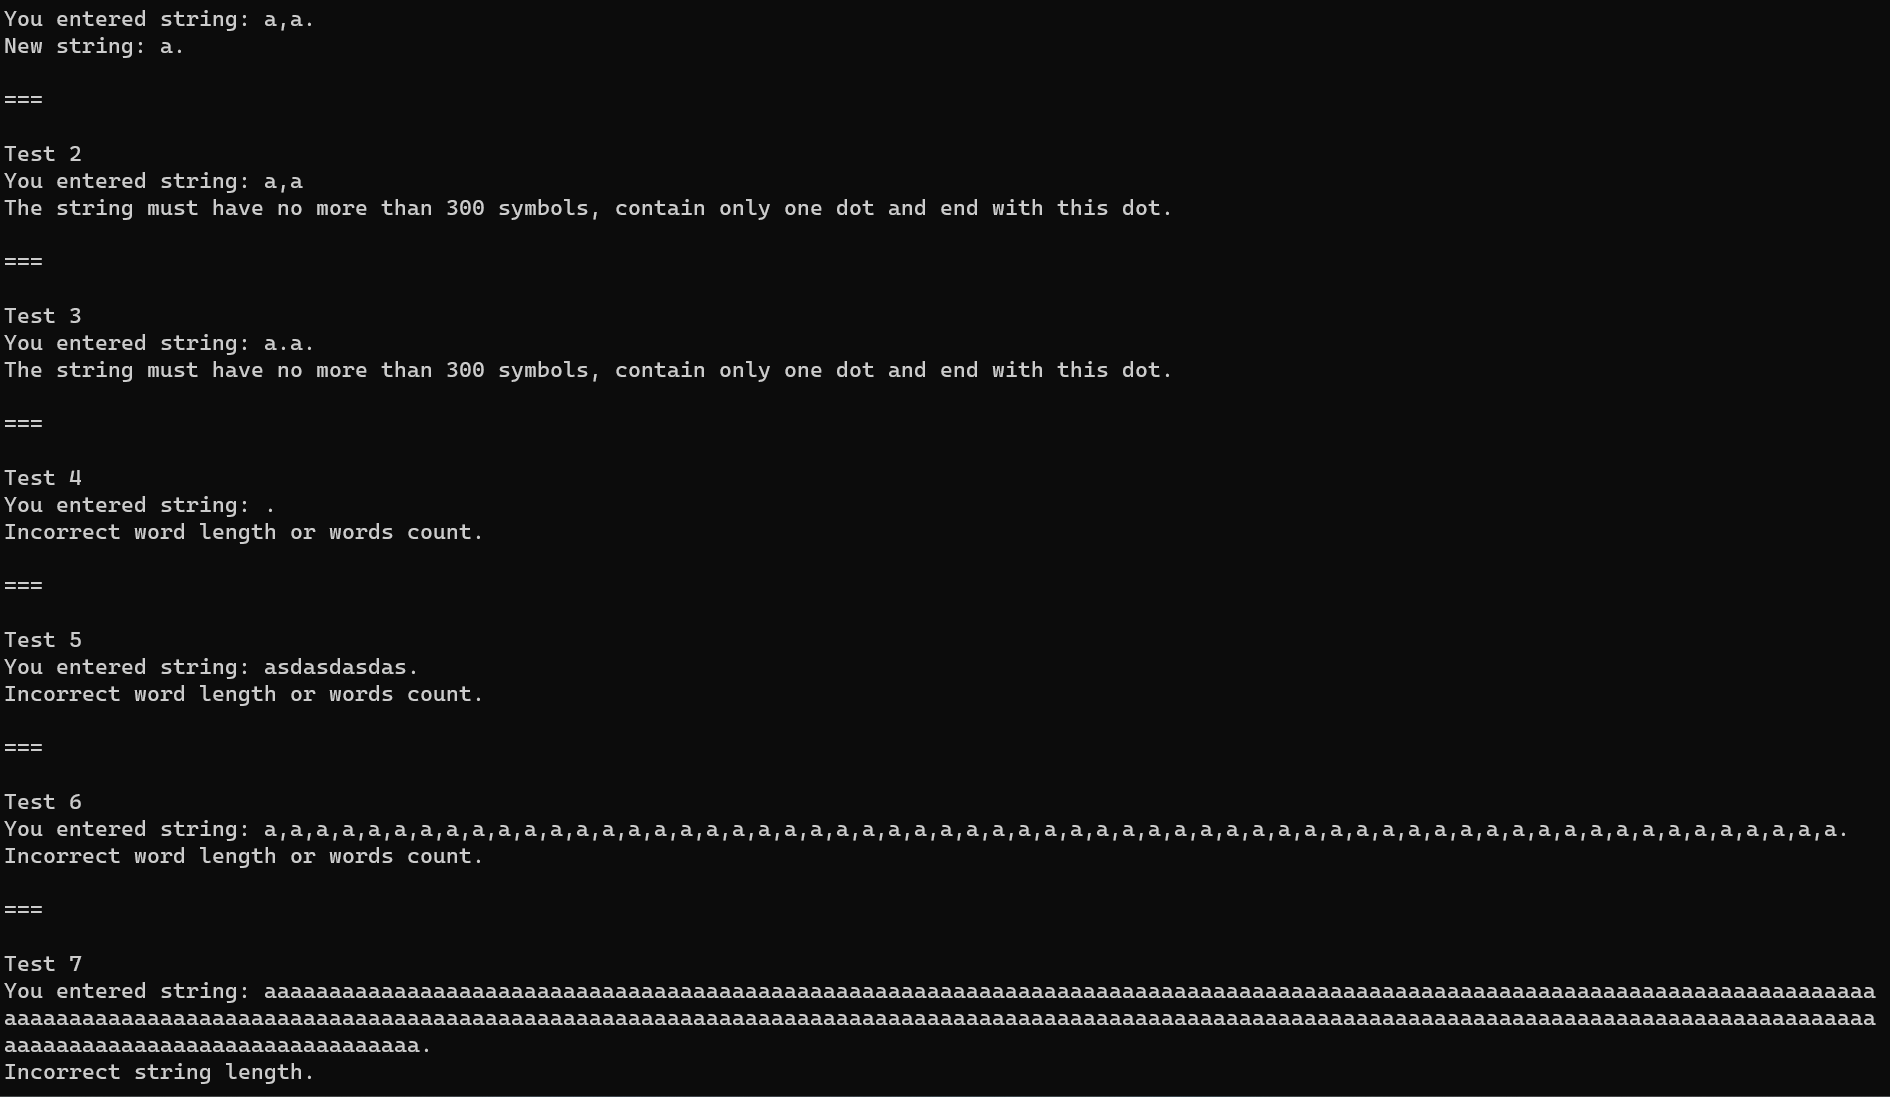
\includegraphics[width=400pt]{tests.png}
	
\end{document}
